\chapter{Introduction\label{cha:introduction}}

Solar power production is highly dependent on weather conditions \cite{lin_temporal_2020, lee_forecasting_2018, jaidee_very_2019, su_machine_2019, jang_solar_2016}. A single cloud can adversely impact the production of a solar farm. Such unreliability in a power production system is undesirable since production must match demand \cite{lee_forecasting_2018}. When solar power production falls, the power demand it was serving must be fulfilled by other means. Fossil fueled power plants are generally kept on standby, waiting to fulfil this demand \cite{lee_forecasting_2018}. These plants often take hours to start, generally pollute more than other plants and are expensive to run \cite{lee_forecasting_2018}.
Reliable and accurate forecasts of the fluctuations in solar power production can give power grid operators notice and insight into future power production \cite{lee_forecasting_2018}. This notice enables planning for the dips in power production and making arrangements for the future. This provides the tools to reduce the cost and pollution of power generation as well as increase the reliability of power delivery to consumers \cite{lee_forecasting_2018}.
Recent advancements in deep learning have unlocked new tools that have been shown to be effective in predicting the future behaviour of a system given enough relevant data.\\

%% \ifdraft only shows the text in the first argument if you are in draft mode.
%% These directions will disappear in other modes.
%\ifdraft{State the objectives of the exercise. Ask yourself:
%  \underline{Why} did I design/create the item? What did I aim to
%  achieve? What is the problem I am trying to solve?  How is my
%  solution interesting or novel?}{}

\section{Background}

\textcolor{red}{TODO: Background on neural networks}\\
Artificial Neural Networks (ANNs), generally known as just Neural Networks (NNs) were first theorized in the 1940s \cite{citation needed}, though it was much later, in the\\
NN function\\


\subsection{LSTMs and GRUs\label{cha:RNN}}
Recurrent Neural Networks (RNNs), especially Gated Recurrent Units (GRUs) and Long-Short Term Memory (LSTM) cells \cite{Goodfellow-et-al-2016} along with more advanced derivatives have been shown to be able to achieve good results when trained on previous weather and power generation data \cite{lin_temporal_2020, lee_forecasting_2018, jaidee_very_2019, su_machine_2019}.
RNNs are a class of deep neural networks where nodes are connected in a temporal sequence, allowing the network to learn time-based data efficiently. LSTMs and GRUs are types of RNNs in which, the nodes in the network have additional stored states controlled by the network via mechanisms that use time delays or feedback loops \cite{Goodfellow-et-al-2016, noauthor_recurrent_2021}.\\

%\ifdraft{Provide background about the subject matter (e.g. How was morse code
%developed?  How is it used today?). 
%This is a place where there are usually many citations.
%It is suspicious when there is not.
%Include the purpose of the different equipment and your design intent. 
%Include references to relevant scientific/technical work and books.
%What other examples of similar designs exist?
%How is your approach distinctive?

%If you have specifications or related standards, these must be
%described and cited also.  As an example, you might cite the specific
%RoboSub competition website (and documents) if working on the lighting system for an AUV\cite{guls2016auvlight}


\subsection{Transformers\label{cha:transformer}}
%Hard to train
%sequential
% -> parallelization hard
%encoder/decoder instead. Attention. 
% Explain enc/dec
% Autoencoders generate same output as the input, so no labeled data is needed -> completely unsupervisd earning.
% Locality a problem with CNNs and RNNs. Can easily find local context but keeping on to context far apart in input is difficult. Enter transformers.
 %Encoder reads blocks of data and uses that and previously generated data as inputs into decoder which generatesdata one point at a time.
 %Attention. How you relate things to each other. i.e. input to output
 %self attention. How do features in the input data relate to each other
 \textcolor{red}{TODO: Make this coherent}
 
Transformers have been used for a while in Natural Language Processing (NLP) and have more recently been used very effectively in forecasting.\cite{vaswani_attention_2017} They can more effectively learn and preserve local context located far apart in the input data. As an example from NLP, the training data can contain multiple cases where time is being told, far apart. A transformer model would then more easily identify that the word “o’clock” is generally preceded by a number, whereas RNNs would be more likely to struggle with such distributed information. This can be applied to our work as similar weather patterns would reoccur days apart and cause a similar effect on measured irradiance at the power station.

\begin{figure}[ht!]
    \centering
    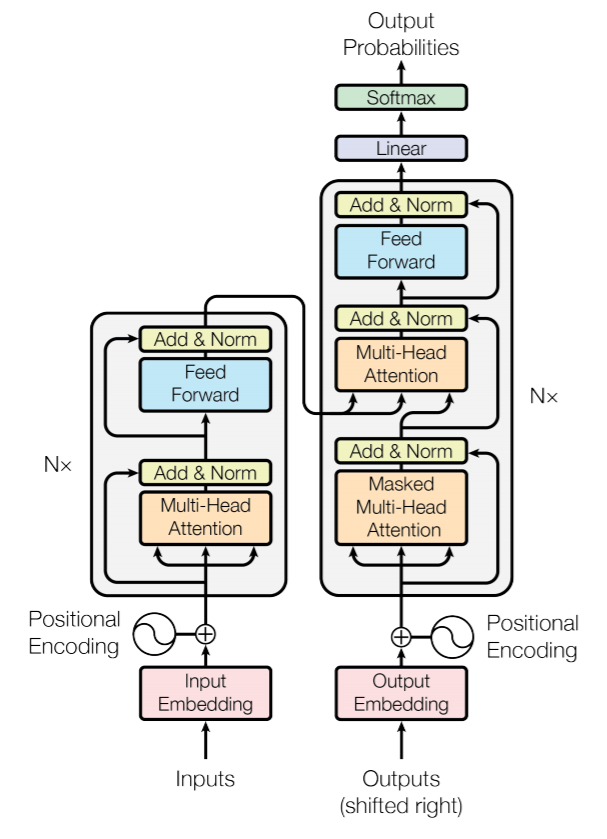
\includegraphics[scale=0.95]{imgs/transformer.png}
    \caption{The transformer architecture.\cite{vaswani_attention_2017}
    \label{fig:transformer}}
\end{figure}



\subsubsection{Encoder/decoder}
Transformers have an encoder/decoder structure. An encoder takes an input sequence and generates an abstract hidden state which the decoder then uses to generate an output sequence. A major advantage of this methodology is that the inputs and outputs do not have to have the same length, whereas the primary limit of the architecture is that all information in the input sequence needs to be represented by a single vector for the decoder to decode. The encoder distils the input down to a much smaller representation, a bottleneck, only containing desired information which the decoder in turn extracts. This is on its own used for tasks like de-noising or colourizing images. 

\begin{figure}[ht!]
    \centering
    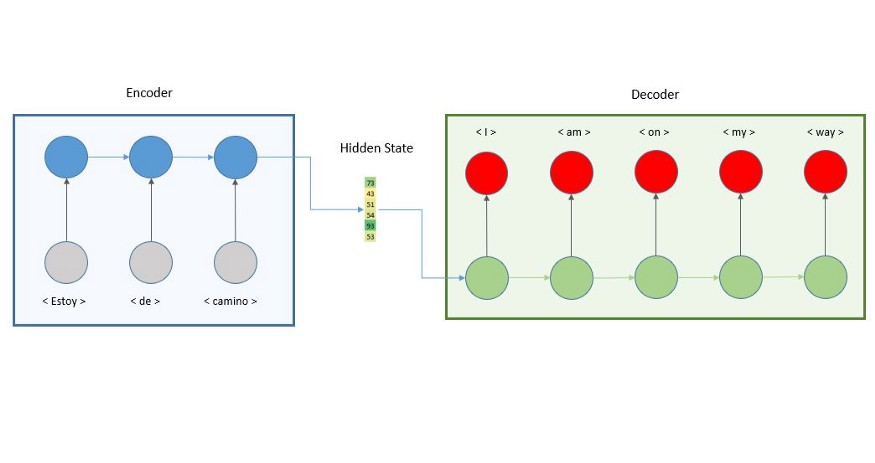
\includegraphics[scale=0.5]{imgs/encoder_decoder.jpeg}
    \caption{The encoder/decoder structure \cite{nechu_what_2020}
    \label{fig:encoder_decoder}}
\end{figure}

\subsubsection{Positional encoding}
Unlike RNNs, the transformer architecture has no recurrence and does inherently track the order of the input data, so positional information has to be injected into the network input for the model to be able to use the positional context of the data.\cite{vaswani_attention_2017}

\subsubsection{Self-attention} We previously discussed transformers' ability to preserve context across the long input sequences. That is thanks to the attention layer. The attention layer encodes an input data point's relevance to the rest of the points in the input sequence. Calling back to the previous NLP example, it encodes the context that the word "o'clock" is relevant to numbers because it is preceded by a number in most inputs.
 
A single attention head can put all the focus on a single element. Multiple attention heads can be used to let the transformer model consider the context of more elements at the same time \cite{rohrer_transformers_2021}.

\subsection{Weather forecasts}
\textcolor{red}{TODO}

\subsection{Previous work}
Lin et al. \cite{lin_temporal_2020} showed that while the more traditional GRUs and LSTMs show good performance on the task, Temporal Convolutional Neural Networks (TCNN) can show even better performance. \textit{"TCNN is a novel convolutional architecture designed for sequential modelling, which combines causal and dilated convolutions
and residual connections"} \cite{lin_temporal_2020}. \\
Jaidee et al. \cite{jaidee_very_2019} showed that LSTMs, GRUs and derivative methods show relatively similar performance for very short-term predictions on the time scale of a few hours. This timescale is where it is critical to accurately predict cloud movements. 
These methods have been taken as far as building genetic algorithms to generate the optimal neural network for the purpose \cite{jaidee_very_2019}. These genetic algorithms operate on the same principles as animal breeding. They generate multiple candidate neural networks and use the best networks as a base to generate new networks for the next generation. This is done for multiple generations and in the end, the best neural network generated is used \cite{jaidee_very_2019}.\\
Su et al. \cite{su_machine_2019} did extensive experimentation on more conventional neural networks and newer, less known networks including  Non-linear Auto Regressive Neural Network (NARXNN), as well as various statistical approaches. When predicting power output, NARXNN takes in the current power output values and considers them as well as the past values of the power output of the system. These experiments showed that NARXNN had the best performance of these, by a rather large margin, and a hybrid method, of the better performing methods, showed even better results \cite{anderson_using_2018}. The statistical methods generally performed significantly worse in predicting the power output. \\
Satellite imagery has been used for predicting solar power output as well. A neural network was trained to predict solar power production, primarily from cloud cover information it learned from these satellite images \cite{jang_solar_2016}.\\
 
\section{Goals}
The methods previously used all have in common that they must effectively predict the weather so they can predict power output.


Here we explore using high-resolution weather forecast data from meteorological models, offloading a majority of this difficult task to the field of meteorology. Instead, we focus on correlating these forecasts with measurements and detecting and reducing temporal and spatial error in the general forecasts using newer methods like Temporal Fusion Transformers.
What is the quality of the predictions this methodology produces? Can we create a model which is useful to power producers in operating their systems more efficiently?


The thesis is structured as follows. First we talked about the motivations and background in the introduction. Next we cover the methods, the data and tools used to achieve these goals. The proceeding chapter contains the results of the work, and finally we discuss the implications, strengths and flaws of the work, future work and end with conclusions.


%Here we explore whether better prediction accuracy can be reached
%if high quality, high resolution weather forecast data is used. This offloads a majority of the difficult task of predicting the weather from the responsibilities of the network. \\
%Can we construct a transformer based neural network which, by utilizing weather forecast data, is superior to neural networks which only utilize historical weather data?\\


%% Glossary is broken, do not use --foley
% \gls{auv}\footnote{Autonomous Undersea Vehicle}.

% Notice that there is now information on the AUV in the Index and Acronyms.
% It isn't in the \gls{glossary} because we didn't put it there.
%\index{AUV}
%}{}


